\section{Transport phenomena in ideal gases}
	A gas molecule has finite mass and random thermal motion. Hence it possesses momentum as well as kinetic energy. Therefore, when a gas moves across different parts of a container, it can transport matter, energy or momentum.
	
	In an equilibrium state, there is no net transfer of matter, energy or momentum. However, if, in a non-equilibrium state, there is macroscopic motion of the gas in a particular direction, the following three cases may occur:
	\begin{enumerate}
		\item \emph{Different parts of the gas move with different velocities.}
		\begin{itemize}
			\item Leads to relative motion between different layers of the gas.
			\item Hence, molecules crossing from faster moving layers transport greater momentum than those crossing from slower moving layers.
			\item The net transport of momentum in a given direction of motion across an imaginary plane is characterized by the \emph{coefficient of viscosity} $\eta$.
		\end{itemize}
		
		\item \emph{Different parts of the gas are at different temperatures.}
		\begin{itemize}
			\item Molecules moving from regions of higher temperature to regions of lower temperature will carry greater thermal energy.
			\item This gives rise to thermal conduction, which is characterized by the thermal conductivity $K$.
		\end{itemize}
		
		\item \emph{Different parts of the gas have different concentrations.}
		\begin{itemize}
			\item Molecules migrating from regions of higher concentration to regions of lower concentration carry matter.
			\item This gives rise to diffusion, which is characterized by the coefficient of diffusion $D$.
		\end{itemize}
	\end{enumerate}
	
	\subsection{Viscosity: Transport of momentum}
		The property of a fluid by virtue of which it opposes the relative motion between adjacent layers is known as \emph{viscosity}. The \emph{coefficient of viscosity} $\eta$ is defined as the tangential force per unit area when a unit velocity gradient exists in a direction perpendicular to the direction of motion.
		\begin{figure}[h!]
			\centering
			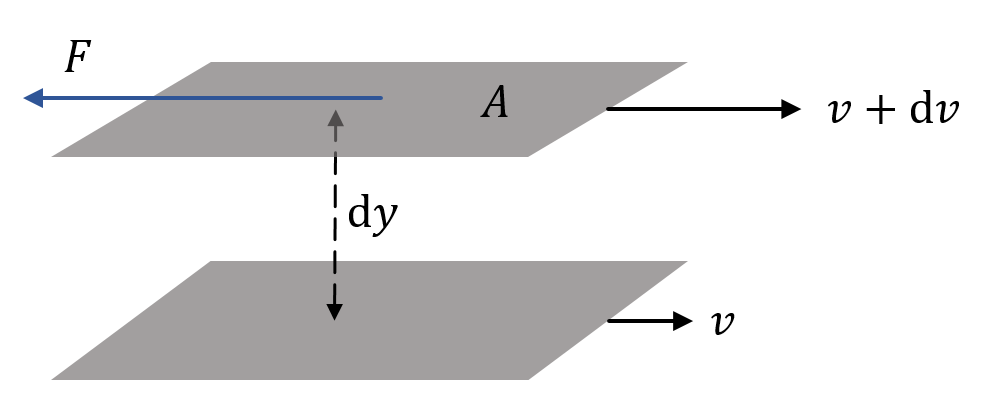
\includegraphics[width=0.5\textwidth]{figures/fig_viscosity-01}
		\end{figure}
		
		Consider two layers of the fluid which are separated by a distance $\dd{y}$, and moving with speeds $v$ and $v+\dd{v}$. Then the velocity gradient between these layers is $\dv{v}{y}$. If $F$ is the viscous force acting on an arbitrary area $A$, then we have
		\begin{align*}
			F=-\eta A\dv{v}{y}
		\end{align*}
	
	\subsection{Thermal conductivity: Transport of energy}
	
	\subsection{Diffusion: Transport of matter}